\begin{figure}[tbp]
\centering
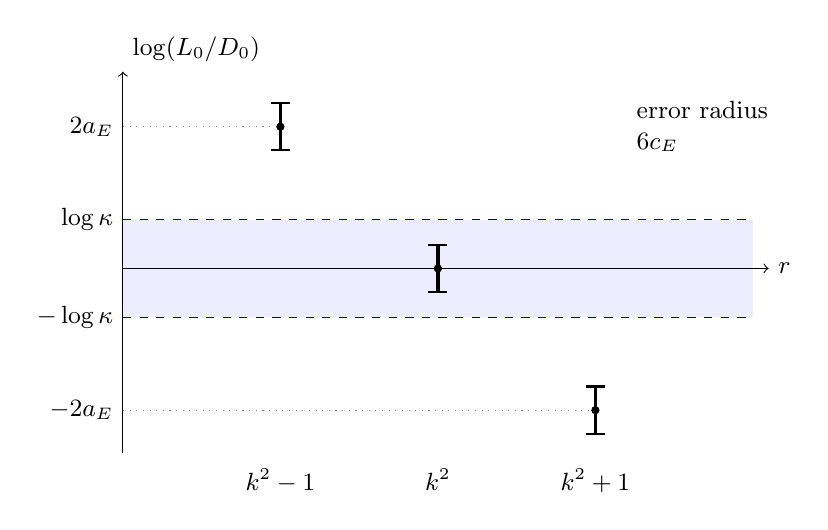
\begin{tikzpicture}[x=1cm,y=1cm,font=\small]
  \fill[blue!7] (1,-.62) rectangle (9,.62);
  \draw[blue!55!black,dashed] (1,.62)--(9,.62);
  \draw[blue!55!black,dashed] (1,-.62)--(9,-.62);
  \draw[->] (1,-2.35)--(1,2.5)
    node[above right] {$\log(L_0/D_0)$};
  \draw[->] (1,0)--(9.2,0) node[right] {$r$};
  \node[left] at (1,.62) {$\log\kappa$};
  \node[left] at (1,-.62) {$-\log\kappa$};
  \draw[gray,dotted] (1,1.8)--(3,1.8);
  \draw[gray,dotted] (1,-1.8)--(7,-1.8);
  \node[left] at (1,1.8) {$2a_E$};
  \node[left] at (1,-1.8) {$-2a_E$};
  \foreach \x/\y in {3/1.8,5/0,7/-1.8}{
    \draw[very thick] (\x,\y-.30)--(\x,\y+.30);
    \draw[thick] (\x-.12,\y-.30)--(\x+.12,\y-.30);
    \draw[thick] (\x-.12,\y+.30)--(\x+.12,\y+.30);
    \fill (\x,\y) circle (1.5pt);
  }
  \node[below] at (3,-2.42) {$k^2-1$};
  \node[below] at (5,-2.42) {$k^2$};
  \node[below] at (7,-2.42) {$k^2+1$};
  \node[right,align=left] at (7.4,1.8) {error radius\\$6c_E$};
\end{tikzpicture}
\caption{The index window, schematically for \(k\ge2\). At index \(r\),
the logarithmic ratio lies within \(6c_E\) of \(2a_E(k^2-r)\).
The choice \(6c_E<\log\kappa<2a_E-6c_E\) puts the entire middle
interval in the admissible band and every other integer-index interval
outside it. The error bars represent bounds, not additional variables.}
\label{fig:height-window}
\end{figure}
